\section{Flussprobleme}

\begin{definition}
    \index{Netzwerk}
    \index{Quelle}
    \index{Ziel}

    Ein \emph{Netzwerk} besteht aus $3$ Komponenten:
    \begin{enumerate}
        \item einem endlichen gerichteten Graph $G = (V, E)$ ohne Schleifen
            (Kanten von $v_i$ zum selben Knoten $v_i$) und ohne parallele Kanten,
        \item einer Funktion $c$, $c:E \rightarrow \mathbb{R}^{+}$, die jeder
            Kante $e \in E$ ihre Kapazität zuordnet,
        \item $2$ ausgezeichneten Knoten $s$ und $t$, genannt \emph{Quelle} und
            \emph{Ziel}. Diese Knoten müssen nicht im Graphentheoretischen Sinne
            Quelle und Senke sein.
    \end{enumerate}

    Soll ein Graph mit parallelen Kanten in ein Netzwerk überführt werden,
    ersetzt man alle parallelen Kanten durch jeweils nur eine Kante. Die
    Kapazität dieser neuen Kante ist gleich der Summe der Kapazitäten der
    Kanten, die sie ersetzt:
    %TODO bild
    
    Schleifen $e = (v, v)$ ergeben im Kontext von Flussproblemen keinen Sinn.
    Falls sie trotzdem in einem Netzwerk dargestellt werden sollen, kann man
    sie durch Kanten $e' = (v, v')$ und $e'' = (v', v)$ zu einem neuen Knoten
    $v'$ darstellen.
    %TODO bild
\end{definition}


\begin{definition}
    \index{Flussfunktion}
    \index{Flusserhaltungsgesetz}
    \index{Fluss!totaler Fluss}

    Eine \emph{Flussfunktion} für ein Netzwerk $(G, c, s, t)$ ist eine Funktion
    $f:E \rightarrow \mathbb{R}$, für die gilt:
    \begin{enumerate}
        \item $0 \leq f(e) \leq c(e)$
        \item sei $\alpha(v) = \{ e: e \text{ führt zu } v \}$, $\beta(v) = \{
            e: e \text{ führt aus } v \}$, $v \in V$ Knoten, dann gilt $\forall v$
            mit $v \neq s$ und $v \neq t$ das \emph{Flusserhaltungsgesetz}:
            $$ \sum_{e \in \alpha(v)} f(e) = \sum_{e \in \beta(v)} f(e) $$
            %TODO bild
    \end{enumerate}

    \noindent
    Sei $f$ eine Flussfunktion, dann heißt $$F = \sum_{e \in \alpha(t)} f(e)
    - \sum_{e \in \beta(t)} f(e)$$ der \emph{totale Fluss} von $f$. Der totale
    Fluss bezieht sich stets auf das -- frei wählbare -- Ziel des Netzwerks
    $t$.
\end{definition}


\begin{bemerkung}
    Eine typische Aufgabe ist es, zu einem Netzwerk eine Flussfunktion $f$ zu
    suchen, so dass ihr totaler Fluss $F$ maximal ist.
\end{bemerkung}


\begin{definition}
    \index{Schnitt}
    \index{Schnitt!Kapazität}

    Sei $S \subseteq V$ mit $s \in S$, $\overline{S} = V \setminus S, t \in
    \overline{S}$.

    $E_{S\overline{S}} = \{ e: \text{ Anfangspunkt von $e \in S$}, \text{
    Endpunkt von $e \in \overline{S}$}\}$

    $E_{\overline{S}S} = \{ e: \text{ Anfangspunkt von $e \in \overline{S}$},
    \text{ Endpunkt von $e \in S$}\}$

    %TODO bild
    
    Der durch $S$ definierte \emph{Schnitt} ist die Menge $E_{S\overline{S}}
    \cup E_{\overline{S}S}$. Die Kapazität des durch $S$ definierten Schnitts
    ist $$c(S) = \sum_{e \in E_{S\overline{S}}} c(e) \qquad \text{(Beachte:
    dies ist die Kapazität in Richtung $\overline{S}$, $t \in \overline{S}$)}$$
\end{definition}


\begin{lemma}
    \label{totalerfluss}
    Sei $N = (G, c, s, t)$ ein Netzwerk, und $f$ eine Flussfunktion für $N$.
    Dann gilt $\forall S \subseteq V$ mit $s \in S$ und $t \notin S$: $$
    F = \sum_{e \in E_{S\overline{S}}} f(e) - \sum_{e \in E_{\overline{S}S}}
    f(e)$$
    Egal welches $S$ man wählt, der totale Fluss (gebunden an $t$) lässt sich
    damit berechnen.
\end{lemma}


\begin{beweis}
    \setcounter{equation}{0}
    \begin{align}
        0 &= \sum_{e \in \alpha(v)} f(e) - \sum_{e \in \beta(v)} f(e) \qquad
          \forall v, v \neq s, v \neq t, \text{ weil $f$ Flussfunktion} \\
        F &= \sum_{e \in \alpha(t)} f(e) - \sum_{e \in \beta(t)} f(e) \qquad
        \text{ Definition von $F$}
    \end{align}

    Addiere Gleichung $(1)$ für alle $v \in \overline{S} \setminus \{t\}$ zu
    Gleichung $(2)$. Auf der linken Seite der Ergebnisgleichung steht $F$. Im
    folgenden bestimmen wir die rechte Seite. Betrachte alle Kanten in $E$: sei
    $e \in E$ mit $x \stackrel{e}{\rightarrow} y$.
    \begin{itemize}
        \item Fall 1: $x, y \in S$: dann kommt $f(e)$ in der Summation nicht
            vor (es wird nur über $v \in \overline{S} \setminus \{t\}$ summiert).
        \item Fall 2: $x, y \in \overline{S}: e \in \alpha(x), e \in \beta(x)$,
            also heben sich die Werte von $f(e)$ bei der Summation gegenseitig auf.
        \item Fall 3: $x \in S, y \in \overline{S}: f(e)$ ist positiv für $y$,
            für $x$ kommt es nicht in der Summation vor, $e \in E_{S\overline{S}}$.
        \item Fall 4: $x \in \overline{S}, y \in S: f(e)$ ist negativ für $x$,
            kommt für $y$ nicht in der Summation vor, $e \in E_{\overline{S}S}$.
    \end{itemize}

    Bei der Summation über die rechte Seite ergibt sich: $$ \sum_{e \in
    E_{S\overline{S}}} f(e) - \sum_{e \in E_{\overline{S}S}} f(e) \qquad
    \text{(Fall 3 - Fall 4)}$$
\end{beweis}


\begin{beispiel}
    Schreibweise: $\nicefrac{c}{f} \qquad \nicefrac{\text{Kapazität}}{\text{Fluss}}$
    %TODO bild
\end{beispiel}


\begin{lemma}
    \label{flusskleinerkap}
    Für jede Flussfunktion $f$ mit totalem Fluss $F$ und für jedes $S \subseteq
    V$ mit $s \in S, t \notin S$ gilt: $F \leq c(S)$.
\end{lemma}


\begin{beweis}
    Aus Lemma \ref{totalerfluss} folgt:
    $$ F_{3.1} = \sum_{e \in E_{S\overline{S}}} f(e) - \sum_{e \in
    E_{\overline{S}S}} \leq \sum_{e \in E_{S\overline{S}}} f(e) \leq \sum_{e
    \in E_{S\overline{S}}} c(e) \stackrel{\text{Def}}{=} c(S)$$
\end{beweis}


\begin{korollar}
    \index{Max Flow Min Cut}
    
    \emph{Max Flow Min Cut-Theorem}: Sei $f$ eine Flussfunktion und $S
    \subseteq V, s \in S, t \notin S$. Wenn $F = c(S)$, dann ist $f$ eine
    Flussfunktion mit maximalem totalen Fluss und die Kapazität des durch $S$
    definierten Schnittes ist minimal.
\end{korollar}


\begin{beweis}
    Sei für ein $f$ und ein $S$ der totale Fluss $F = c(S)$. Sei $f'$ eine
    andere Flussfunktion mit totalem Fluss $F'$. Aus Lemma
    \ref{flusskleinerkap} folgt: $F' \leq c(S) = F$, also ist $F$ maximal.

    Sei $S' \subseteq V$ mit $s \in S', t \notin S'$. Dann gilt:
    $\underset{=c(S)}{F} \leq c(S)$, also ist $c(S)$ minimal.
\end{beweis}


\begin{definition}
    \index{Anreicherungspfad}
    \index{Augmenting Path}

    Gegeben sei ein Netzwerk $(G, c, s, t)$ und eine Flussfunktion $f$ für
    dieses Netzwerk. Ein \emph{Anreicherungspfad} (Augmenting Path) ist ein
    einfacher Pfad oder Weg von $s$ nach $t$, der nicht notwendigerweise
    gerichtet ist, und für den gilt: Sei $e$ eine Kante auf diesem Weg: 

    \begin{center}
        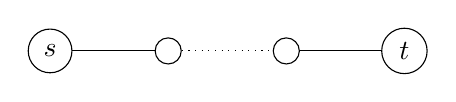
\begin{tikzpicture}
            \node (s) at (0, 0) [draw, shape=circle] {$s$};
            \node (v1) at (1.5, 0) [draw, shape=circle] {};
            \node (v2) at (3, 0) [draw, shape=circle] {};
            \node (t) at (4.5, 0) [draw, shape=circle] {$t$};

            \draw (s) -- (v1);
            \draw (v2) -- (t);
            \draw[dotted] (v1) -- (v2);
        \end{tikzpicture}
    \end{center}

    \begin{itemize}
        \item Fall 1: $e$ ist eine \emph{Vorwärtskante}, d.h. \\
            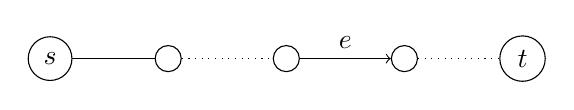
\begin{tikzpicture}
                \node (s) at (0, 0) [draw, shape=circle] {$s$};
                \node (v1) at (1.5, 0) [draw, shape=circle] {};
                \node (v2) at (3, 0) [draw, shape=circle] {};
                \node (v3) at (4.5, 0) [draw, shape=circle] {};
                \node (t) at (6, 0) [draw, shape=circle] {$t$};

                \draw (s) -- (v1);
                \draw[->] (v2) -- (v3);
                \draw[dotted] (v3) -- (t);
                \draw[dotted] (v1) -- (v2);

                \node (e) at (3.75, 0.2) {$e$}; 
            \end{tikzpicture} \\
            dann muss $f(e) < c(e)$ sein.
        \item Fall 2: $e$ ist eine \emph{Rückwärtskante}, d.h. \\
            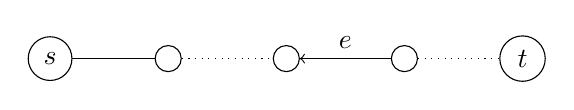
\begin{tikzpicture}
                \node (s) at (0, 0) [draw, shape=circle] {$s$};
                \node (v1) at (1.5, 0) [draw, shape=circle] {};
                \node (v2) at (3, 0) [draw, shape=circle] {};
                \node (v3) at (4.5, 0) [draw, shape=circle] {};
                \node (t) at (6, 0) [draw, shape=circle] {$t$};

                \draw (s) -- (v1);
                \draw[<-] (v2) -- (v3);
                \draw[dotted] (v3) -- (t);
                \draw[dotted] (v1) -- (v2);

                \node (e) at (3.75, 0.2) {$e$};
            \end{tikzpicture} \\
            dann muss $f(e) > 0$ sein.
    \end{itemize}
\end{definition}


\begin{beispiel}
    %TODO bild und so
\end{beispiel}


\begin{definition}
    \index{Vorwärtsmarkierung}
    \index{Rückwärtsmarkierung}

    Eine \emph{Vorwärtsmarkierung} des Knoten $v$ durch die Kante 
    \begin{tikzpicture}[baseline]
        \node (u) at (0, 0) {$u$};
        \node (v) at (1.5, 0) {$v$};
        \draw[->] (u) -- (v);
        \node (e) at (0.75, 0.2) {$e$};
    \end{tikzpicture}
    ist anwendbar, wenn \begin{enumerate}
        \item $u$ markiert ist und $v$ nicht, und
        \item $f(e) > 0$.
    \end{enumerate}
    $v$ erhält dann die Markierung ``$e$'' (Name der Kante). 
    
    Eine \emph{Rückwärtsmarkierung} des Knoten $v$ durch die Kante 
    \begin{tikzpicture}[baseline]
        \node (u) at (0, 0) {$u$};
        \node (v) at (1.5, 0) {$v$};
        \draw[<-] (u) -- (v);
        \node (e) at (0.75, 0.2) {$e$};
    \end{tikzpicture}
    ist anwendbar, wenn \begin{enumerate}
        \item $u$ markiert ist und $v$ nicht, und
        \item $f(e) > 0$.
    \end{enumerate}
    $v$ erhält dann die Markierung ``$e$''. 

    Im 1. Fall, also bei Vorwärtsmarkierung, wird $\Delta(e) = c(e) - f(e)$. Im
    2. Fall wird $\Delta(e) = f(e)$. In beiden Fällen ist $\Delta(e) > 0$.
\end{definition}


\begin{definition}
    \index{Ford-Fulkerson-Algorithmus}

    \emph{Algorithmus von Ford und Fulkerson zur Bestimmung einer Flussfunktion
    mit maximalem totalen Fluss}. Gegeben sei ein Netzwerk $(G, c, s, t)$ und
    eine Flussfunktion $f$ für dieses Netzwerk. Der folgende Algorithmus
    verändert $f$ mit dem Ziel, den totalen Fluss zu maximieren.

    \begin{enumerate}
        \item Setze $f(e) := 0 \qquad \forall e \in E$
        \item Kennzeichne $s$ als ``markiert'' und alle anderen Knoten als
            ``unmarkiert''
        \item Suche einen Knoten $v$, der vorwärts oder rückwärts markiert
            werden kann. Gibt es keinen solchen Knoten, dann halte an. Das damit
            gefundene $f$ hat maximalen totalen Fluss. Gibt es einen solchen Knoten
            $v$, dann markiere $v$ mit der Kante $e$, die zur Markierung geführt
            hat. Ist $v = t$, dann gehe zu Schritt 4, ansonsten zu Schritt 3.
        \item Starte bei $t$ und rekonstruiere mittels der Markierungen den
            ``Weg'', auf dem man von $s$ nach $t$ gelangt ist. Dies sei 
            \begin{center}
                \begin{tipi}
                    \node (s) at (0, 0) {$s=v_0$};
                    \node (v1) at (1.5, 0) {$v_1$};
                    \node (v2) at (3, 0) {$v_{e-1}$};
                    \node (v3) at (4.5, 0) {$v_l=t$};

                    \draw (s) -- (v1);
                    \draw (v2) -- (v3);
                    \draw[dotted] (v1) -- (v2);

                    \node (e1) at (3.75, 0.2) {$e_l$};
                    \node (e2) at (0.75, 0.2) {$e_1$};
                \end{tipi} 
            \end{center}
            Sei $\Delta = min(\{\Delta(e_i): 1 \leq i \leq l \} )$. Ist $e_i$
            eine Vorwärtskante, so setze $f(e_i) := f(e_i) + \Delta$,
            andernfalls $f(e_i) := f(e_i) - \Delta$.
        \item Gehe zu Schritt 2.
    \end{enumerate}
\end{definition}


\begin{beispiel}
    In diesem Beispiel wird der Ford-Fulkerson-Algorithmus auf ein Netzwerk
    angewendet. Die folgende Abbildung zeigt das Netzwerk vor dem ersten
    Schritt.
    \begin{center}
        \begin{tipi}
            \node (s) at (0, 0) [draw, shape=circle] {$s$};
            \node (a) at (1.25, 1.25) [draw, shape=circle] {$a$};
            \node (b) at (3, 1.25) [draw, shape=circle] {$b$};
            \node (c) at (1.25, -1.25) [draw, shape=circle] {$c$};
            \node (d) at (3, -1.25) [draw, shape=circle] {$d$};
            \node (t) at (4.25, 0) [draw, shape=circle] {$t$};

            \draw[->] (s) -- (a);
            \draw[->] (a) -- (b);
            \draw[<-] (a) -- (d);
            \draw[->] (b) -- (t);
            \draw[->] (d) -- (t);
            \draw[->] (c) -- (d);
            \draw[->] (s) -- (c);
            \draw[->] (b) -- (c);

            \node (l1) at (0.75, 0.4) {$e_1$};
            \node (l2) at (0.75, -0.4) {$e_2$};
            \node (l3) at (2.125, 1.05) {$e_3$};
            \node (l6) at (2.125, -1.05) {$e_6$};
            \node (l8) at (3.5, -0.4) {$e_8$};
            \node (l4) at (2.75, -0.4) {$e_4$};
            \node (l5) at (1.55, -0.4) {$e_5$};
            \node (l7) at (3.5, 0.4) {$e_7$};

            \node(f1) at (0.25, 0.75) {$\nicefrac{15}{0}$};
            \node(f2) at (0.25, -0.75) {$\nicefrac{4}{0}$};
            \node(f6) at (2.125, -1.55) {$\nicefrac{10}{0}$};
            \node(f3) at (2.125, 1.55) {$\nicefrac{12}{0}$};
            \node(f8) at (3.9, -0.9) {$\nicefrac{10}{0}$};
            \node(f7) at (3.8125, 0.8125) {$\nicefrac{7}{0}$};
            \node(f4) at (1.55, 0.4) {$\nicefrac{5}{0}$};
            \node(f5) at (2.75, 0.4) {$\nicefrac{3}{0}$};
        \end{tipi}
    \end{center}

    ``Wege'' in den Iterationsschritten, gefundenes $\Delta$, neue Flusswerte:
    \begin{enumerate}
        \item 
            \begin{tipi}[baseline]
                \node (s) at (0, 0) {$s$};
                \node (c) at (1.5, 0) {$c$};
                \node (d) at (3, 0) {$d$};
                \node (a) at (4.5, 0) {$a$};
                \node (b) at (6, 0) {$b$};
                \node (t) at (7.5, 0) {$t$};

                \draw[->] (s) -- (c);
                \draw[->] (c) -- (d);
                \draw[->] (d) -- (a);
                \draw[->] (a) -- (b);
                \draw[->] (b) -- (t);

                \node (l1) at (0.75, 0.2) {$e_2$};
                \node (l2) at (2.25, 0.2) {$e_6$};
                \node (l3) at (3.75, 0.2) {$e_4$};
                \node (l4) at (5.25, 0.2) {$e_3$};
                \node (l5) at (6.75, 0.2) {$e_7$};

                \node (delta) at (-0.8, -0.3) {$\Delta(e):$};
                \node (d1) at (0.75, -0.3) {$4$};
                \node (d2) at (2.25, -0.3) {$10$};
                \node (d3) at (3.75, -0.3) {$5$};
                \node (d4) at (5.25, -0.3) {$12$};
                \node (d5) at (6.75, -0.3) {$7$};
            \end{tipi} \\
            $\Rightarrow \Delta = 4$ \\
            $\Rightarrow e_2 \rightarrow \nicefrac{4}{4} \qquad e_3 \rightarrow
            \nicefrac{12}{4} \qquad e_6 \rightarrow \nicefrac{10}{4} \qquad e_7
            \rightarrow \nicefrac{7}{4} \qquad e_4 \rightarrow \nicefrac{5}{4}$ \\
            $\Rightarrow F = 4$

        \item \begin{tipi}[baseline]
                \node (s) at (0, 0) {$s$};
                \node (c) at (1.5, 0) {$a$};
                \node (d) at (3, 0) {$b$};
                \node (a) at (4.5, 0) {$c$};
                \node (b) at (6, 0) {$b$};
                \node (t) at (7.5, 0) {$t$};

                \draw[->] (s) -- (c);
                \draw[->] (c) -- (d);
                \draw[->] (d) -- (a);
                \draw[->] (a) -- (b);
                \draw[->] (b) -- (t);

                \node (l1) at (0.75, 0.2) {$e_1$};
                \node (l2) at (2.25, 0.2) {$e_2$};
                \node (l3) at (3.75, 0.2) {$e_5$};
                \node (l4) at (5.25, 0.2) {$e_6$};
                \node (l5) at (6.75, 0.2) {$e_8$};

                \node (delta) at (-0.8, -0.3) {$\Delta(e):$};
                \node (d1) at (0.75, -0.3) {$15$};
                \node (d2) at (2.25, -0.3) {$8$};
                \node (d3) at (3.75, -0.3) {$3$};
                \node (d4) at (5.25, -0.3) {$6$};
                \node (d5) at (6.75, -0.3) {$10$};
            \end{tipi} \\
            $\Rightarrow \Delta = 3$ \\
            $\Rightarrow e_1 \rightarrow \nicefrac{15}{3} \qquad e_3
            \rightarrow \nicefrac{12}{7} \qquad e_5 \rightarrow \nicefrac{3}{3}
            \qquad e_6 \rightarrow \nicefrac{10}{7} \qquad e_8 \rightarrow
            \nicefrac{10}{3}$ \\
            $\Rightarrow F = 7$

        \item \begin{tipi}[baseline]
                \node (s) at (0, 0) {$s$};
                \node (c) at (1.5, 0) {$a$};
                \node (d) at (3, 0) {$b$};
                \node (a) at (4.5, 0) {$t$};

                \draw[->] (s) -- (c);
                \draw[->] (c) -- (d);
                \draw[->] (d) -- (a);

                \node (l1) at (0.75, 0.2) {$e_1$};
                \node (l2) at (2.25, 0.2) {$e_3$};
                \node (l3) at (3.75, 0.2) {$e_7$};

                \node (delta) at (-0.8, -0.3) {$\Delta(e):$};
                \node (d1) at (0.75, -0.3) {$12$};
                \node (d2) at (2.25, -0.3) {$5$};
                \node (d3) at (3.75, -0.3) {$3$};
            \end{tipi} \\
            $\Rightarrow \Delta = 3$ \\
            $\Rightarrow e_1 \rightarrow \nicefrac{15}{6} \qquad e_3
            \rightarrow \nicefrac{12}{10} \qquad e_7 \rightarrow \nicefrac{7}{7}$\\
            $\Rightarrow F = 10$

        \item \begin{tipi}[baseline]
                \node (s) at (0, 0) {$s$};
                \node (c) at (1.5, 0) {$a$};
                \node (d) at (3, 0) {$d$};
                \node (a) at (4.5, 0) {$t$};

                \draw[->] (s) -- (c);
                \draw[->] (c) -- (d);
                \draw[->] (d) -- (a);

                \node (l1) at (0.75, 0.2) {$e_1$};
                \node (l2) at (2.25, 0.2) {$e_4$};
                \node (l3) at (3.75, 0.2) {$e_8$};

                \node (delta) at (-0.8, -0.3) {$\Delta(e):$};
                \node (d1) at (0.75, -0.3) {$9$};
                \node (d2) at (2.25, -0.3) {$4$};
                \node (d3) at (3.75, -0.3) {$7$};
            \end{tipi} \\
            $\Rightarrow \Delta = 4$ \\
            $\Rightarrow e_1 \rightarrow \nicefrac{15}{10} \qquad e_4
            \rightarrow \nicefrac{5}{0} \qquad e_8 \rightarrow \nicefrac{10}{7}$\\
            $\Rightarrow F = 14$

        \item Nach $a$ und $b$ kann kein weiterer Knoten markiert werden, der
        Algorithmus bricht ab. $f$ hat jetzt maximalen totalen Fluss.
    \end{enumerate}
\end{beispiel}


\begin{lemma}
    Nach jedem Durchlauf durch einen der Iterationsschritte des Algorithmus
    gilt: das aktuell berechnete $f$ ist eine Flussfunktion.
\end{lemma}


\begin{beweis}
    Trivial für die Schritte 1, 2, 3 und 5. Schritt 4:

    Sei $f$ die Flussfunktion vor Eintritt in Schritt 4 und $f'$ die in Schritt
    4 berechnete Funktion. $f$ erfülle die Bedingungen
    \begin{enumerate}
        \item $0 \leq f(e) \leq c(e)$
        \item $\forall v \in V, v \neq s, v \neq t: \sum_{e \in \alpha(v)} f(e)
            = \sum_{e \in \beta(v)} f(e)$
    \end{enumerate}
    In Schritt 4 wird ein Anreicherungspfad rekonstruiert, dies sei: 
    \begin{center}
        \begin{tipi}
            \node (s) at (0, 0) {$s=v_0$};
            \node (v1) at (1.5, 0) {$v_1$};
            \node (v2) at (3, 0) {};
            \node (v3) at (4.5, 0) {$v_k=t$};

            \draw (s) -- (v1);
            \draw (v2) -- (v3);
            \draw[dotted] (v1) -- (v2);

            \node (e1) at (3.75, 0.2) {$e_k$};
            \node (e2) at (0.75, 0.2) {$e_1$};
        \end{tipi} 
    \end{center}
    Die Definition von $\Delta(e)$ und $\Delta$ garantiert, dass $0 \leq f'(e)
    \leq c(e)$. Zu zeigen bleibt das Flusserhaltungsgesetz für $f'$. Wir müssen
    nur die Knoten anschauen, die auf dem Weg liegen, d.h. $v_1, \dots,
    v_{k-1}$. Sei $v_i$ einer dieser Knoten. Es können folgende Fälle
    auftreten: 
    \begin{itemize}
        \item Fall 1: 
            \begin{tipi}[baseline]
                \node (v0) at (0, 0) {};
                \node (vi) at (2, 0) {$v_i$};
                \node (v1) at (4, 0) {};

                \draw[->] (v0) -- (vi);
                \draw[->] (vi) -- (v1);

                \node (ei) at (1, 0.2) {$e_i$};
                \node (li) at (1, -0.3) {$\in \alpha(v_i)$};
                \node (ei1) at (3, 0.2) {$e_{i+1}$};
                \node (li1) at (3, -0.3) {$\in \beta(v_i)$};
            \end{tipi} \\
            $\Delta$ wird zu beiden Kantenflüssen addiert -- zu $\sum_{e \in
            \alpha(v)} f(e)$ und zu $\sum_{e \in \beta(v)} f(e)$.
        
        \item Fall 2: 
            \begin{tipi}[baseline]
                \node (v0) at (0, 0) {};
                \node (vi) at (2, 0) {$v_i$};
                \node (v1) at (4, 0) {};

                \draw[->] (v0) -- (vi);
                \draw[<-] (vi) -- (v1);

                \node (ei) at (1, 0.2) {$e_i$};
                \node (li) at (1, -0.3) {$\in \alpha(v_i)$};
                \node (ei1) at (3, 0.2) {$e_{i+1}$};
                \node (li1) at (3, -0.3) {$\in \alpha(v_i)$};
            \end{tipi} \\
            $\Delta$ wird zur Summe addiert und (wegen Rückwärtskante) subtrahiert.
        
        \item Fall 3: 
            \begin{tipi}[baseline]
                \node (v0) at (0, 0) {};
                \node (vi) at (2, 0) {$v_i$};
                \node (v1) at (4, 0) {};

                \draw[<-] (v0) -- (vi);
                \draw[->] (vi) -- (v1);

                \node (ei) at (1, 0.2) {$e_i$};
                \node (li) at (1, -0.3) {$\in \beta(v_i)$};
                \node (ei1) at (3, 0.2) {$e_{i+1}$};
                \node (li1) at (3, -0.3) {$\in \beta(v_i)$};
            \end{tipi} \\
            Analog zu Fall 2.
                \item Fall 4: 
            \begin{tipi}[baseline]
                \node (v0) at (0, 0) {};
                \node (vi) at (2, 0) {$v_i$};
                \node (v1) at (4, 0) {};

                \draw[<-] (v0) -- (vi);
                \draw[<-] (vi) -- (v1);

                \node (ei) at (1, 0.2) {$e_i$};
                \node (li) at (1, -0.3) {$\in \beta(v_i)$};
                \node (ei1) at (3, 0.2) {$e_{i+1}$};
                \node (li1) at (3, -0.3) {$\in \alpha(v_i)$};
            \end{tipi} \\
            Analog zu Fall 1.
    \end{itemize}
\end{beweis}
\begin{lemma}
Hält der Algorithmus von Fud/Fulkerson an, dann besitzt die zu diesem Zeitpunkt berechnete Flußfunktion f maximalen totalen Fluß.
\end{lemma}
\begin{beweis}
Wenn der Algorithmus anhält, dann tut er dies in Schritt 3 und t wurde nicht erreicht.  Sei S die Menge der Knoten, die beim letztes Markieren markiert wurden.  Auf jeden Fall ist s $\in$ S und $t \notin S$, $\overline{S} := (V,S)$.

Sei $x \rightarrow (e)y \in E_{S\overline{S}}$, dann ist f(e) = c(e) weil sonst entlang dieser kante die Markierung festgesetzt werden könnte.  x<-(p)y $\in E_{S\overline{S}}$, dann muss $f(e)=0$.  

Mit Lemma 3.1 folgt F=$\sum_{e \in E_{S\overline{S}}} f(e) - \sum_{e \in E_{\overline{S}S}} f(e) =
\sum_{e \in E_{S\overline{S}}} c(e) = c(S)$

Mit Lemma 3.3 folgt F maximal.
\end{beweis}

\begin{lemma}
Ist $c:= E \rightarrow \mathbb{N} $, so hält der Algorithmus immer an.
\end{lemma}

\begin{beweis}
ist $c:= E \rightarrow \mathbb{N} $ so wird in jedem Durchlauf der totale Fluß um eine natürliche Zahl $\Delta$ erhöht.  Andererseits gilt $F \leq c(S)$ für eine beliebige Menge $S \subseteq V$, $s \in S$, $t \notin S$
\end{beweis}

\begin{beispiel}
Frage: c: E $\rightarrow$ Reele Zahlen : V

Beispiel: Kosten können sehr hoch werden im Fall $c:E \rightarrow \mathbb{N} $
%					a		
%	10^6/0			10^6/0
%s			1/0				t			F = 2*10^6
%	10^6/0			10^6/0
%				b

1. Markierung: $ s \rightarrow a \rightarrow b \rightarrow t, \Delta = 1$

2. Markierung: $ s \rightarrow b \rightarrow a \rightarrow t, \Delta = 1$

insgesamt $2*10^6$ Markierungssequenzen, d.h. Abhängigkeit von der kapazität.
\end{beispiel}

\begin{definition}
Satz von Edmond und karp:

Verwendet BFS beim Markieren und wählt jeweils den kürzesten Anreichungspfad, dann terminiert der Algorithmus in $O(|V|^3*E)$ Schritten. (Vorausgesetzt die vorkommenden reellen Zalen können jeweils in einem Schritt bearbeitet werden.

\end{definition}

\begin{beispiel}
x sei große Zahl, $x \in \mathbb{N}$, $\phi:= ( \sqrt{5}-1)/2$ (Lösung von $x^2+x-1=0$).  

Insbesondere gilt: $\phi^2+ \phi-1=0$, also $\phi^(k+1)+ \phi^k = \phi(k-1)$, $k \ge 1$
%				a
%							  x/phi->
%	x->			1/phi<-			
%s	  x/1->		b						t
%				1/1-phi->	  x/1->
%				c	
%	x->			phi/phi<-	 x->
%	
%	
%			d

$F= 2x +1$

$1+2* \sum_{k=1}^{\infty} \phi^k = 1 + 2*(1/(1-\phi)) = 4 + \sqrt{5} <7$

Typ0: Weg $s \rightarrow b \rightarrow c \rightarrow t : \Delta =1$

Typ1: Weg $s \rightarrow d \rightarrow c \rightarrow b \rightarrow a \rightarrow t 1: \Delta = \phi, 2:\Delta = 1-\phi = \phi^2$

Typ2: Weg $s->b->c<-d->t : \Delta = \phi$

Typ3: Weg $s->a<-b->c->t : \Delta = 1:\phi^2$

Reihung 0,1,2,1,3

Berechnet:$ \Delta =1, \Delta = \phi, \Delta = \phi, \Delta = \phi^2, \Delta = \phi^2$
\end{beispiel}
\begin{definition}
Sei e eine Kante mit Flußwert $f(e)$.  e heißt nützlich von u nach v, wenn gilt:
\begin{enumerate}
	\item $u \rightarrow^e$ und $f(e) < c(e)$
	\item $u \leftarrow^e v$ und $f(e) > 0$
\end{enumerate}
Eine Schichtung für ein Netzwerk (mit $G=(V,E)$, $c:E \rightarrow \mathbb{R}$, $s,t \in V$) und eine Flußfunktion $f$ ist definiert wie folgt:
\begin{enumerate}
	\item $V_{0}:= {s}$, $i:=0$
	\item T:={$v:v \notin V_{j}$ für $j \le i$ und es existiert eine nützliche Kante von einem Knoten aus $V_{i}$ zu v}
	\item ist $T = \emptyset$ dann ist der jetzige totale Fluß (d.h. der von $f$) maximal, halte an.
	\item Ist $t \in T$, setzte $l_{i} = i+1$, $V_{l} = {t}$, halte an
	\item $V_{i+1} := T$, $i:=i+1$ und gehe zu 2)
\end{enumerate}
\end{definition}
\begin{beispiel}
	\begin{center}
        \begin{tipi}
            \node (s) at (0, 0) [draw, shape=circle] {$s$};
            \node (b) at (1.25, 1.25) [draw, shape=circle] {$b$};
            \node (c) at (3, 1.25) [draw, shape=circle] {$c$};
            \node (d) at (1.25, -1.25) [draw, shape=circle] {$d$};
            \node (e) at (3, -1.25) [draw, shape=circle] {$e$};
            \node (t) at (4.25, 0) [draw, shape=circle] {$t$};

            \draw[->] (s) -- (b);
            \draw[->] (s) -- (d);
            \draw[->] (b) -- (d);
            \draw[->] (b) -- (c);
            \draw[->] (c) -- (d);
            \draw[->] (d) -- (e);
            \draw[->] (c) -- (t);
            \draw[->] (e) -- (t);
			\draw[->] (e) -- (c);

            \node (l1) at (0.75, 0.4) {$e_1$};
            \node (l2) at (0.75, -0.4) {$e_2$};
            \node (l3) at (2.125, 1.05) {$e_4$};
            \node (l6) at (2.125, -1.05) {$e_6$};
            \node (l8) at (3.5, -0.4) {$e_8$};
            \node (l4) at (2.75, -0.4) {$e_9$};
            \node (l5) at (1.0, 0.0) {$e_3$};
            \node (l7) at (3.5, 0.4) {$e_7$};
			\node (l9) at (2.125, 0.4) {$e_5$};

            \node(f1) at (0.25, 0.75) {$\nicefrac{5}{1}$};
            \node(f2) at (0.25, -0.75) {$\nicefrac{4}{1}$};
            \node(f6) at (2.125, -1.55) {$\nicefrac{3}{1}$};
            \node(f4) at (2.125, 1.55) {$\nicefrac{3}{1}$};
            \node(f8) at (3.9, -0.9) {$\nicefrac{5}{1}$};
            \node(f7) at (3.8125, 0.8125) {$\nicefrac{3}{1}$};
            \node(f3) at (1.55, 0.4) {$\nicefrac{1}{0}$};
            \node(f9) at (3.30, 0.0) {$\nicefrac{1}{0}$};
			\node(f5) at (2.1, -0.53) {$\nicefrac{2}{0}$};
        \end{tipi}
    \end{center}
	Fuer dieses Beispiel sollten die Studenten die Schichtenbildung durchfuehren.
\end{beispiel}